\normaltrue \difficilefalse \tdifficilefalse
\correctionfalse
%\UPSTIidClasse{11} % 11 sup, 12 spé
%\newcommand{\UPSTIidClasse}{11}

\exer{Hemostase -- Stabilité$\star$ \label{C2:03:stab:61}}

\setcounter{numques}{0}
\UPSTIcompetence[2]{C2-03}
\index{Compétence C2-03}
\index{Schéma-blocs}
\index{Stabilité}

%%%%%%%%%%%%%%%%%%%%%%%%%%%%%%%


\ifprof
\else
La modélisation de l'asservissement de position est donnée par le schéma-bloc ci-dessous dans lequel $K_2 = 2,78 \cdot 10^{-2} \text{N}^{-1}$, $K_1 = \SI{856}{s^{-1}}$, $T_m= 3\cdot  10^{-2} s$.

Le couple résistant $C_r$ est constant et vaut $C_{r0} = 2,7 \cdot 10^{-3} \text{Nm}$.


\begin{center}
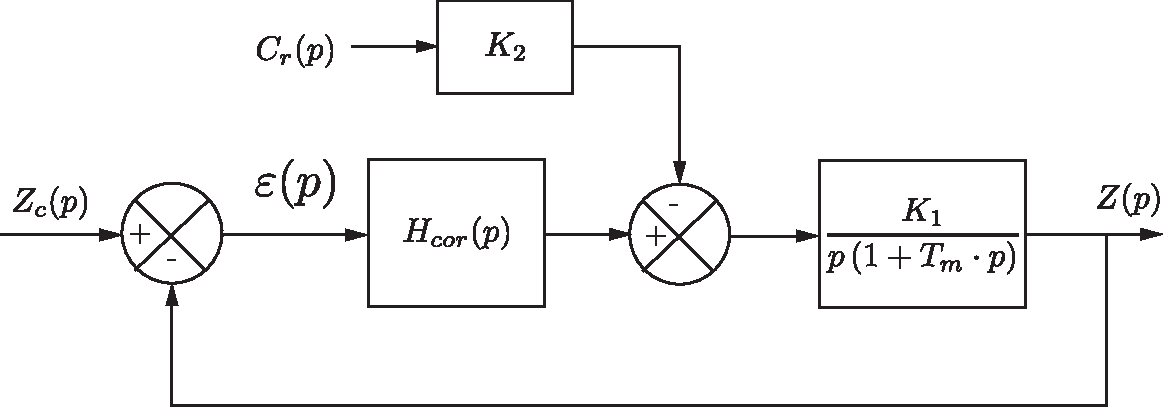
\includegraphics[width=0.7\linewidth]{64_01.pdf}
\end{center}

On suppose le correcteur proportionnel : $H_{\text{cor}}(p)=K_p$.

Les performances du système sont détaillées dans le diagramme des exigences partiel.% (figure \ref{req}). 


\begin{center}
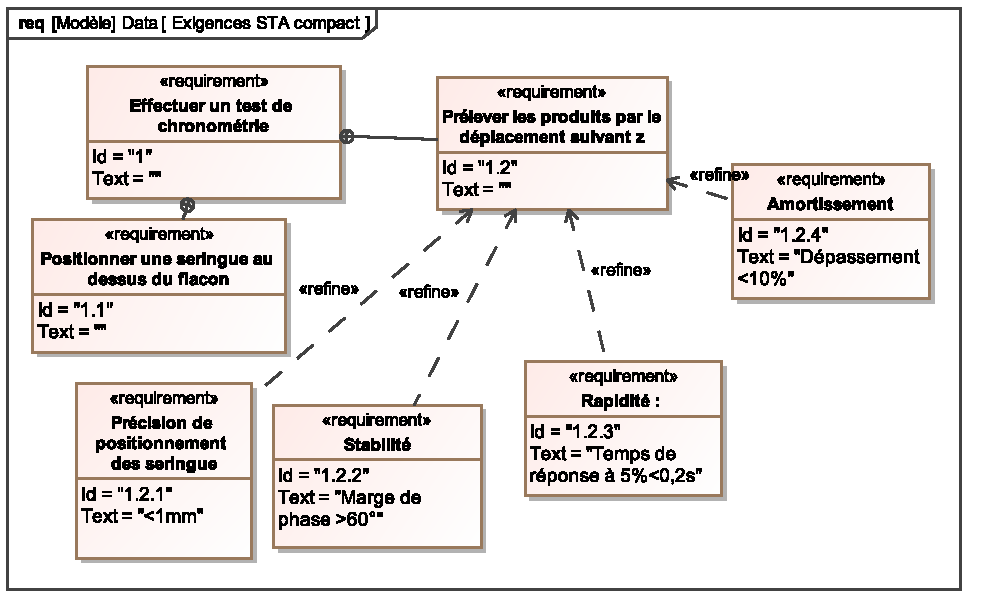
\includegraphics[width=\linewidth]{req.pdf}
\end{center}



\fi
\question{Déterminer l'expression de la fonction de transfert en boucle ouverte $H_{\text{bo}}(p)=\left(\frac{Z(p)}{\varepsilon(p)}\right)_{C_r(p)=0}$ ainsi que la fonction de transfert $H_{\text{cr}}(p)=\left(\frac{Z(p)}{C_r(p)}\right)_{Z_c=0}$.}
\ifprof
%\begin{corrige}~\\

$H_{\text{bo}}(p) = H_{\text{cor}}(p) \dfrac{K_1}{p\left(1+T_m p\right)}$ $=  \dfrac{K_1 K_p}{p\left(1+T_m p\right)}$.

$H_{\text{cr}}(p)= -K_2\dfrac{\dfrac{K_1}{p\left(1+T_m p\right)}}{1+H_{\text{cor}}(p) \dfrac{K_1}{p\left(1+T_m p\right)}}$
$= -K_2\dfrac{K_1}{p\left(1+T_m p\right)+H_{\text{cor}}(p) K_1}$
$= -\dfrac{K_1K_2}{p\left(1+T_m p\right)+K_p K_1}$
%\end{corrige}
\else
\fi

\question{Déterminer l'erreur statique pour une entrée de type échelon d'amplitude $Z_{c0}$ dans l'hypothèse d'une perturbation nulle ($C_{r0}$). Déterminer ensuite l'erreur due à une perturbation constante $C_{r0}$, dans le cas d'une
consigne de position nulle ($Z_c=0$). En déduire la valeur de $K_p$ pour satisfaire le critère de précision du cahier des charges.}
\ifprof
%\begin{corrige}
Exprimons $\varepsilon(p)$ en fonction de $Z_c(p)$ et $C_{r}(p)$ :

$
\varepsilon(p)=Z_c(p)-Z(p) = Z_c(p)- \left(\varepsilon(p) H_{\text{cor}}(p)-   K_2 C_r(p)\right) \dfrac{K_1}{p\left(1+T_m p\right)}$

$\Leftrightarrow \varepsilon(p)\left(1 +  H_{\text{cor}}(p)\dfrac{K_1}{p\left(1+T_m p\right)} \right) 
= Z_c(p) + K_2 C_r(p) \dfrac{K_1}{p\left(1+T_m p\right)}$

$\Leftrightarrow \varepsilon(p)  = 
Z_c(p)\dfrac{1}{1 +  H_{\text{cor}}(p)\dfrac{K_1}{p\left(1+T_m p\right)}} 
+   K_2 C_r(p) \dfrac{K_1}{p\left(1+T_m p\right)} \dfrac{1}{1 +  H_{\text{cor}}(p)\dfrac{K_1}{p\left(1+T_m p\right)}}$

$\Leftrightarrow \varepsilon(p)  = 
Z_c(p)\dfrac{{p\left(1+T_m p\right)}}{{p\left(1+T_m p\right)} +  H_{\text{cor}}(p){K_1}} 
+  K_2 C_r(p)  \dfrac{K_1}{p\left(1+T_m p\right) +  H_{\text{cor}}(p){K_1}}$


En prenant une entrée échelon et une perturbation échelons, on a $Z_c(p) = \dfrac{Z_{c0}}{p}$ et 
$C_{r}(p) = \dfrac{C_{r0}}{p}$.

On a donc $\lim\limits_{t\to +\infty} \varepsilon(t)=\lim\limits_{p\to 0} p\varepsilon(p)$
$=  \lim\limits_{p\to 0} Z_{c0}\dfrac{{p\left(1+T_m p\right)}}{{p\left(1+T_m p\right)} +  H_{\text{cor}}(p){K_1}} 
+   K_2 C_{r0}  \dfrac{K_1}{p\left(1+T_m p\right) +  H_{\text{cor}}(p){K_1}} $ $ =   \dfrac{K_2 C_{r0}}{ K_p}$.

AN : $\varepsilon_s < \SI{1}{mm}$
$\Leftrightarrow \dfrac{K_2 C_{r0}}{ K_p} < \SI{1}{mm}$  
$\Leftrightarrow 
2,78 \cdot 10^{-2} \times 2,7 \cdot 10^{-3} \times 10^3<  K_p$  soit $K_p >0,08$.
%\end{corrige}
\else
\fi


\question{Sur le document réponse %de la figure (\ref{bode_bo}) 
compléter les diagrammes de Bode en gain et en phase de $H_{\text{bo}}(p)$ pour $K_p$ déterminé précédemment. Indiquer si le critère de stabilité est satisfait en justifiant votre démarche par des tracés nécessaires.}
\ifprof
%\begin{corrige}~\\
En ajoutant le gain de 0,08, il faut translater la courbe de gain vers le bas de 22 dB.

\begin{center}
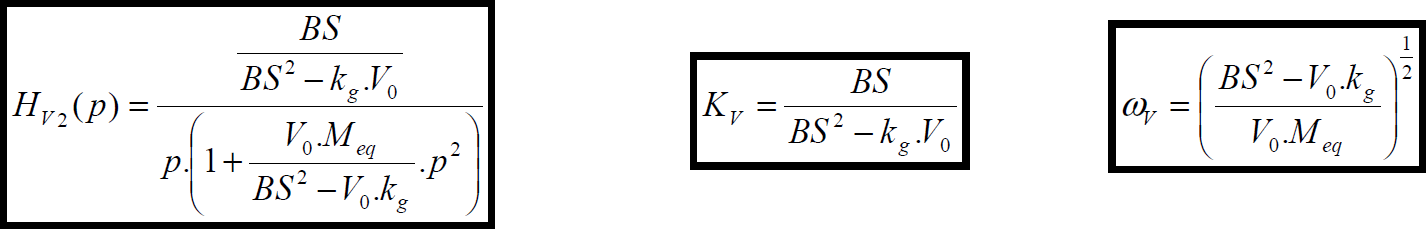
\includegraphics[width=.70\linewidth]{cor_06}
\end{center}

La marge de phase est supérieure à 60\degres.
%\end{corrige}
\else
\fi

Afin d'améliorer le comportement, on implante un correcteur Proportionnel Intégral ayant pour fonction de transfert : $H_{\text{cor}}(p)=\frac{K_p\left(1+T_i\cdot p\right)}{T_i\cdot p}$ avec $K_p=1$ et $T_i = \SI{1}{s}$.

\question{Tracer le diagramme de Bode de la fonction de transfert en boucle ouverte avec ce correcteur avec $K_p=1$ et $T_i = \SI{1}{s}$.}% sur la figure \ref{bode_bo_PI}.}
\ifprof
%\begin{corrige}
%\end{corrige}
\else
\fi

\question{On souhaite une marge de phase d'au moins $60^{\circ}$. Proposer un réglage de $K_p$ pour satisfaire au cahier des charges.}% Justifier vos calculs par les tracés nécessaires sur la figure \ref{bode_bo_PI}.}
\ifprof
%\begin{corrige}
%\end{corrige}
\else
\fi

\question{La figure suivante %\ref{reponse_2nd_ordre} 
donne la réponse à un échelon de position de \SI{50}{mm} avec trois types de correcteurs. Vérifier qu'elle est conforme au cahier des charges. Justifier clairement vos réponses en donnant les valeurs numériques pour chaque critère.}
\ifprof

%\begin{corrige} ~\\
\begin{center}
\begin{tabular}{|l|c|c|c|}
\hline
 & P & PI & PID \\  \hline
 Temps de réponse < à 5\,\% < \SI{0,2}{s} &Ok & Ok & Ok \\ \hline
Précision < \SI{1}{mm} & Ok (?) & Ok & Ok \\ \hline
 Dépassement < à 10\,\% < \SI{0,2}{s} & Pas Ok & Pas Ok & Ok \\ \hline
\end{tabular}
\end{center}

\begin{center}
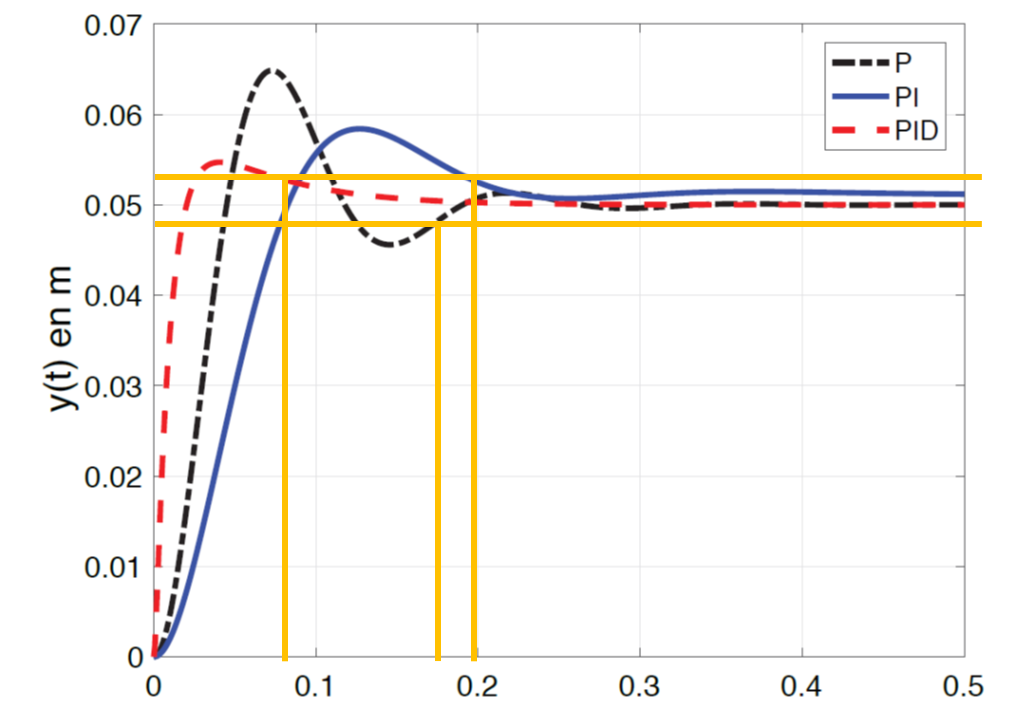
\includegraphics[width=.5\linewidth]{cor_07}
\end{center}

%\end{corrige}
\else
\fi

\ifprof
\else
%\begin{figure}[!htb]
\begin{center}
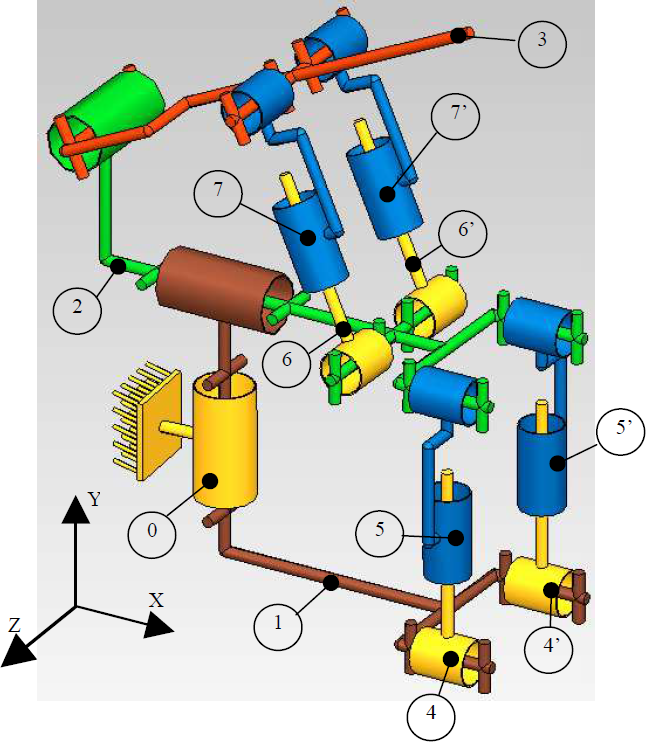
\includegraphics[width=.70\linewidth]{64_02}
%\caption{Réponse à un échelon de position de $50 mm$ avec trois correcteurs P(question 2) PI (question 5) et PID (déterminé numériquement)\label{reponse_2nd_ordre}}
\end{center}
%\end{figure}
\fi

\question{Analyser les résultats à l'aide du diagramme de Bode de la FTBO corrigé avec un PID optimisé.}% (figure \ref{bode_pid}.)}
\ifprof
%\begin{corrige}~\\

\begin{center}
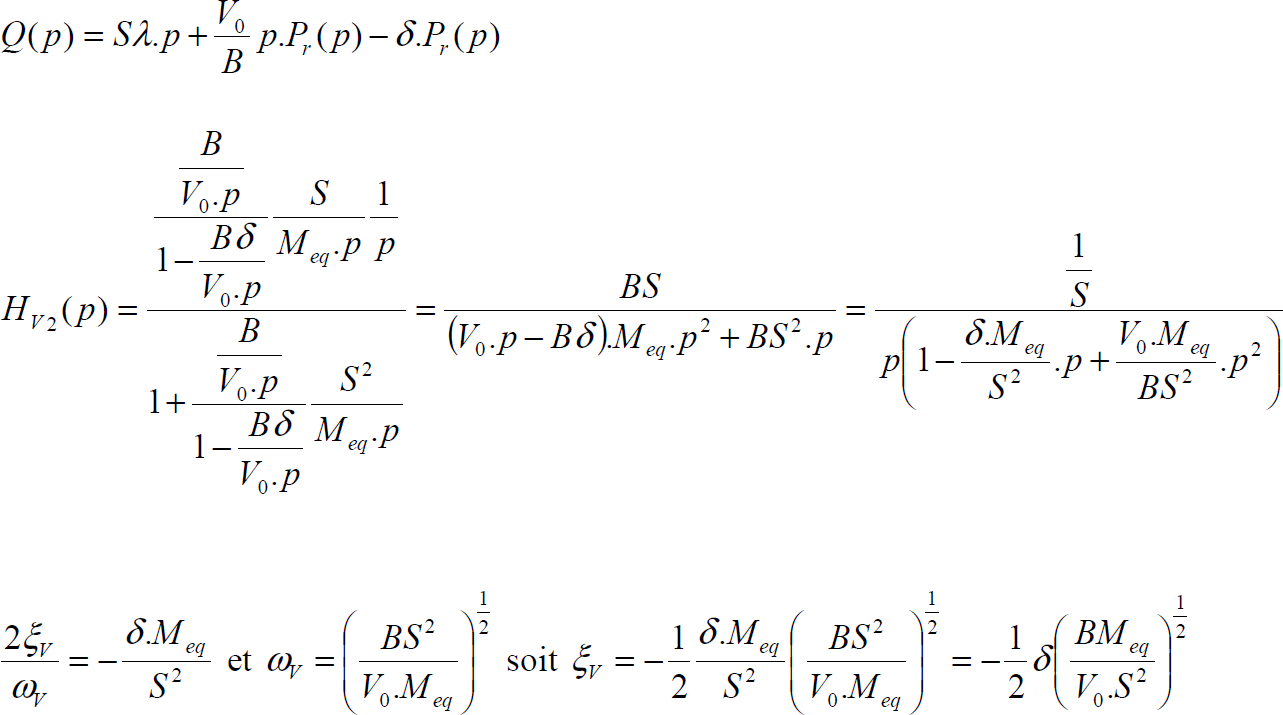
\includegraphics[width=.5\linewidth]{cor_08}
\end{center}

La marge de phase est supérieure à 60\degres.

%\end{corrige}
\else
\fi


\ifprof
\else
\begin{center}
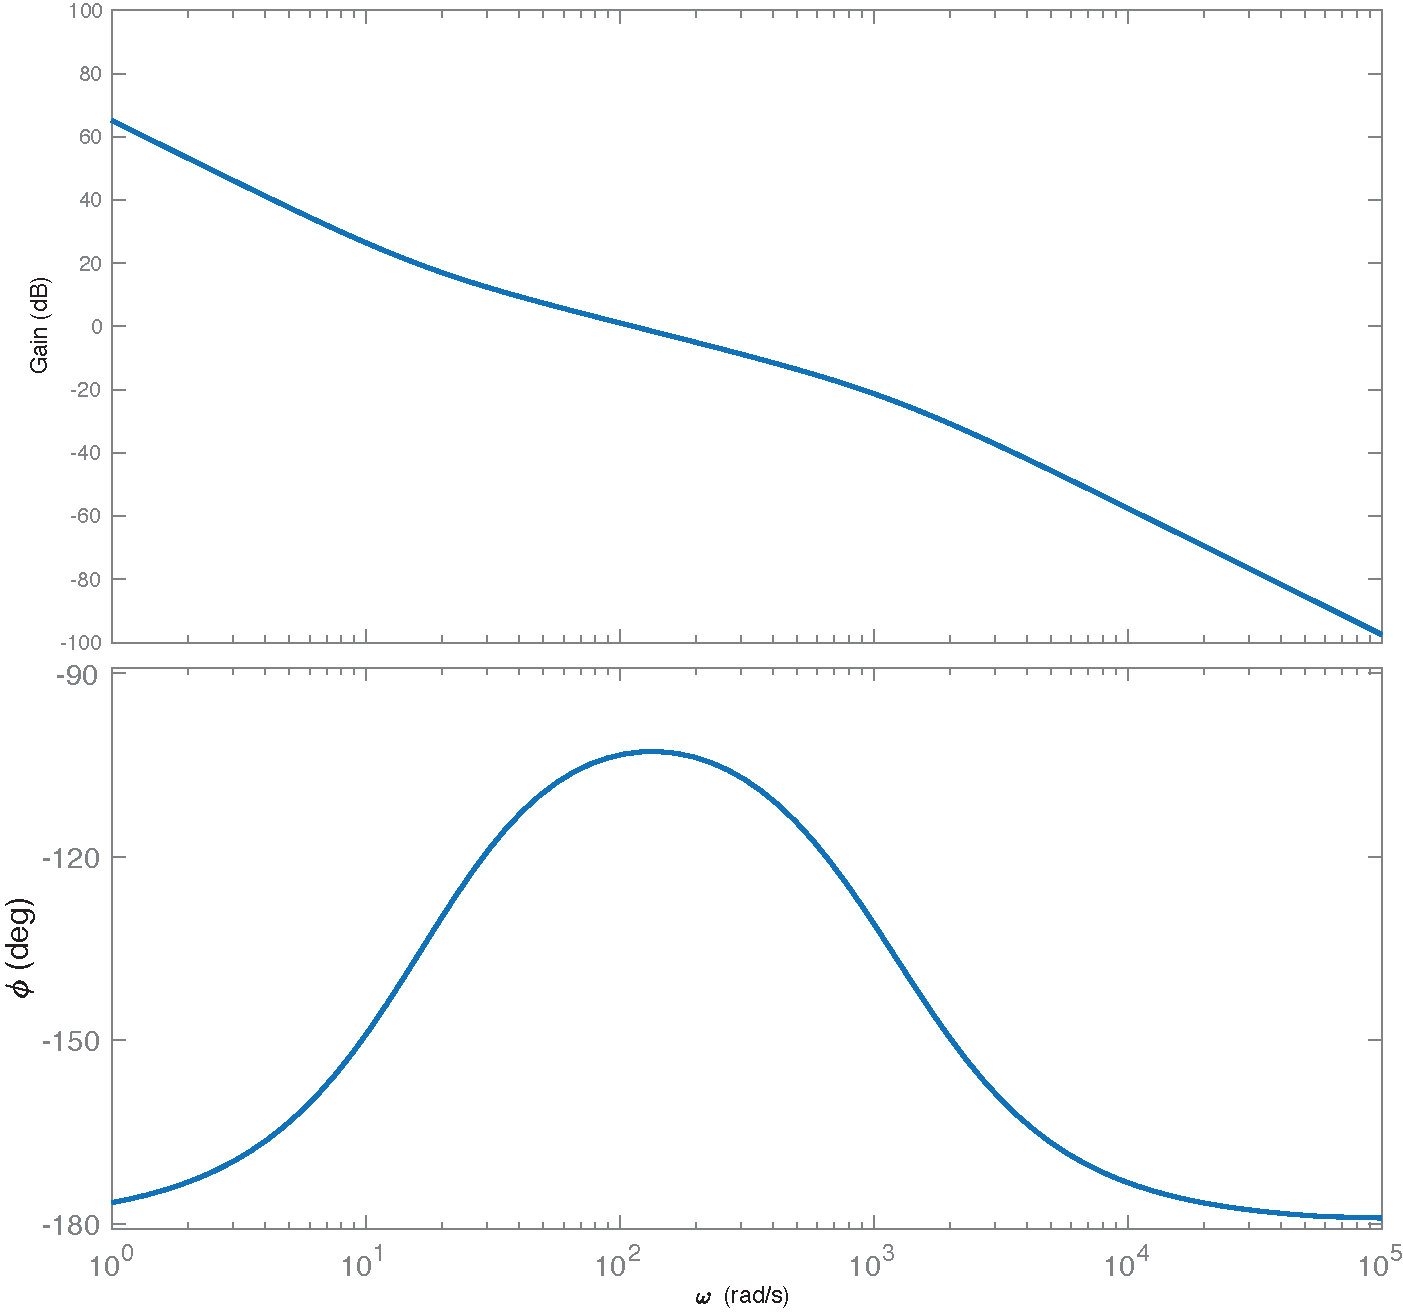
\includegraphics[width=.70\linewidth]{64_03}
%\caption{Diagramme de Bode de $H_{bo}(p)$ avec un correcteur PID pour $K_p=0,19$, $K_i=2,1$ et $K_d=0,0038$\label{bode_pid}}
\end{center}
\fi


%%%%%%%%%%%%%%%%%%%%%%%%%%%%%%%
 

\ifprof
\else
%
%\noindent\footnotesize
%\fbox{\parbox{.9\linewidth}{
%Éléments de corrigé : 
%\begin{enumerate}
%  \item $k_{BO}=\sqrt{2}{\tau_m}$.
%    \item $k_c=\dfrac{\sqrt{2}N}{\tau_m k_m k_r} = 471,1$.
%    \item $\varepsilon_s=0$.
%\end{enumerate}}}
%\normalsize

\begin{flushright}
\footnotesize{Corrigé  voir \ref{C2:03:stab:61}.}
\end{flushright}%
\fi